\documentclass[11pt,a4paper,twoside]{article}

% Basic packages
\usepackage{amsmath, amssymb}
\usepackage{graphicx}
\usepackage{xcolor}
\usepackage{geometry}
\usepackage{float}
\usepackage{wrapfig}
\usepackage{titlesec}
\usepackage{fancyhdr}
\usepackage{caption}
\usepackage{subcaption}
\usepackage{hyperref}
\usepackage{fontspec}
\usepackage{nomencl}
\usepackage{multicol}
\usepackage{etoolbox}
\usepackage{multirow}
\usepackage{csquotes}
\usepackage{tcolorbox}
\usepackage{listings}

% Restore \underbar and \underline before loading sectsty
\let\oldunderbar\underbar
\let\oldunderline\underline
\usepackage{sectsty} % Custom section styles

% Fonts
\setmainfont{Poppins} % Main font
\newfontfamily\titlesfont{Anonymous Pro} % Titles font
\setmonofont{Anonymous Pro} % Monospace font

% Bibliography
\usepackage[backend=biber, style=ieee, citestyle=numeric]{biblatex}
\addbibresource{references.bib}

% Define colors
\definecolor{cherenkovblue}{RGB}{55, 139, 230} % Signature blue
\definecolor{darkgreen}{RGB}{34,139,34}  % Comments (green)
\definecolor{darkorange}{RGB}{255,140,0} % Strings (orange)
\definecolor{blue}{RGB}{30,144,255}      % Keywords (blue)
\definecolor{lightgray}{RGB}{245,245,245} % Background


% Itemize lists use bullets
\renewcommand{\labelitemi}{\textbullet}

% Adjust default font sizes
\renewcommand{\normalsize}{\fontsize{9}{11}\selectfont}
\renewcommand{\small}{\fontsize{8}{10}\selectfont}
\renewcommand{\footnotesize}{\fontsize{7}{9}\selectfont}

% Section formatting
\makeatletter
\renewcommand{\section}{\@startsection {section}{1}{\z@}%
  {-3.5ex \@plus -1ex \@minus -.2ex}%
  {2.3ex \@plus.2ex}%
  {\titlesfont\fontsize{14}{16}\bfseries\color{cherenkovblue}\MakeUppercase}}
\makeatother

\subsectionfont{\titlesfont\fontsize{12}{14}\bfseries\color{cherenkovblue}}

% Customize spacing
\setlength{\parskip}{6pt}
\setlength{\parindent}{0pt}
\setlength{\itemsep}{4pt}

% Fancy headers & footers
\fancypagestyle{plain}{\fancyhf{}} % Default plain style
\fancypagestyle{post-index}{
    \fancyhf{}
    \fancyhead[LE]{\textit{Simone Pagliuca, et al.}}
    \fancyhead[RO]{\textit{Title or whatever}}
    \fancyfoot[LE,RO]{\thepage}
    \renewcommand{\headrulewidth}{0.4pt}
    \renewcommand{\footrulewidth}{0.4pt}
    \setlength{\headheight}{14pt}
}

% Code Formatting
\lstdefinestyle{custombox}{
    backgroundcolor=\color{gray!10},
    frame=single,
    rulecolor=\color{black},
    basicstyle=\ttfamily\small, % Monospace font
    breaklines=true,
    captionpos=b,
    numbers=left,
    numberstyle=\tiny\color{gray},
    keywordstyle=\color{blue}\bfseries,  % Bold blue keywords
    commentstyle=\color{darkgreen}\itshape, % Italic green comments
    stringstyle=\color{darkorange}, % Orange strings
    showstringspaces=false,
    tabsize=4
}
\lstset{style=custombox}

% Box styles
\tcbset{
    boxstyle/.style={
        colframe=cherenkovblue,
        colback=white,
        coltitle=white,
        fonttitle=\bfseries,
        rounded corners,
        width=\textwidth,
        boxrule=0.75mm,
        arc=2mm,
        toptitle=2mm,
        bottomtitle=2mm,
        sharp corners=downhill
    }
}

% Document begins
\begin{document}

% Title Page
\thispagestyle{plain}

% Title with Titles Font (Anonymous Pro)
{\titlesfont\fontsize{18}{28}\textbf{\color{cherenkovblue}{GENETIC ALGORITHM: \\ IMPLEMENTATION AND OPTIMIZATION}}}\\
{\titlesfont\fontsize{10}{12}\color{cherenkovblue} Nuclear Engineering - Politecnico di Milano}\\

\vspace{-10pt}

% Author information with Main Font (Poppins)
{\normalsize\textbf{Pagliuca Simone}} \\
{\footnotesize\textit{simone1.pagliuca@mail.polimi.it}} \\

\vspace{15pt}

% Course and Academic Year
{\footnotesize\textbf{Course:} Advanced Topics for Nuclear Engineering}\\
{\footnotesize\textbf{Academic year:} 2024/2025}

% Horizontal rule
\vspace{10pt}
\centerline{\rule{1.0\textwidth}{0.4pt}}

\vspace{15pt}

% Abstract with Titles Font for Heading, Main Font for Body
\begin{minipage}{1\textwidth}
    \noindent {\titlesfont\fontsize{12}{14}\textbf{\color{cherenkovblue} Abstract:}} 
    {\normalsize
    The objective of this project is to explore the implementation and optimization of a Genetic Algorithm (GA) solver to minimize the Styblinski-Tang function. This report details the approach taken for coding the GA solver, a parametric study on its performance, and the results obtained. The Styblinski-Tang function, with a known global minimum, serves as a benchmark for evaluating the accuracy and efficiency of the algorithm.
    }
\end{minipage}

\vspace{20pt}

% Key-words box with Titles Font
\begin{tcolorbox}[arc=0pt, boxrule=0pt, colback=cherenkovblue!60, width=\textwidth, colupper=white]
    {\titlesfont\fontsize{10}{10}\textbf{Key-words:}} Genetic Algorithm, Optimization, Algorithm Performance
\end{tcolorbox}

\vspace{12pt}

% Nomenclature

\newpage

\newpage

% Table of Contents
\tableofcontents
\newpage
\pagestyle{post-index}

% Main Content
\graphicspath{{images/}}
\sloppy

\section{Introduction}

For the safe operation of a nuclear reactor, it is essential to have precise knowledge of the reactivity characteristics of all control units. The calibration of a control rod enables a quantitative assessment of the reactivity variation induced by the insertion of a neutron absorber into the reactor core.

This study aims to present and validate the subcritical control rod calibration procedure for the TRIGA Mark II Reactor located at LENA, Pavia. 

The validation process involves developing a Monte Carlo simulation model using the SERPENT code to estimate the control rod worth. 
The numerical results are then subjected to experimental validation through dedicated measurements in the reactor facility, ensuring the reliability of the proposed methodology.

\subsection{The subcritical method for CR calibration}
The subcritical method for control rod calibration relies on the principles of subcritical multiplication, establishing a correlation between reactivity insertion due to control rod movement and a measurable parameter dependent on neutron flux.

By employing an external neutron source, the reactor can sustain a stable neutron flux even while remaining in a subcritical state ($k_{\text{eff}} < 1$). One of the primary advantages of this method is its safety, as the reactor never reaches a critical or supercritical state during the experiment. Additionally, the procedure is relatively straightforward and requires significantly shorter measurement times compared to alternative calibration techniques.

However, the method has certain limitations, it requires a prior reference calibration, typically obtained using a different approach, and the accuracy of measurements is constrained by the low power levels at which the reactor operates during the experiment. 

Furthermore, the precision of the results is influenced by the characteristics of the neutron source and the measurement chain employed.

Despite these challenges, the subcritical method remains a valuable and practical technique for control rod calibration, particularly in TRIGA reactor kinetics studies, where its simplicity and safety provide key advantages.

\newpage
\subsection{TRIGA Reactor Description}

The TRIGA (Training, Research, Isotope production, General Atomics) reactor family consists of 66 nuclear research reactors operating in 23 countries, with power ratings ranging from 20 kW to 14 MW. These reactors are primarily used for education and training, materials testing, medical applications, and detector calibration.

The TRIGA Mark II reactor located in Pavia, Italy, reached its first criticality in 1965 and represents one of the latest designs in the TRIGA series. A defining characteristic of TRIGA reactors is their inherent safety, ensuring a self-regulating response to reactivity insertion events. This design principle eliminates the need for complex external safety systems, making them particularly suitable for training environments.

\blockquote{{TRIGA reactors} should be safe even in the hands of young undergraduate students.}{Frederic de Hoffmann \footnote{Frederic de Hoffmann (1924–1989) was a nuclear physicist involved in the Manhattan Project and later played a role in founding General Atomics. See:~\parencite{DeHoffmann1989}.}}

This philosophy aligns well with their role in academic and research institutions.

The inherent safety of TRIGA reactors is achieved through three fundamental safety functions:
\begin{itemize}
    \item \textbf{Control}: Regulating reactivity.
    \item \textbf{Cooling}: Managing heat removal via natural convection.
    \item \textbf{Containment}: Preventing the release of radioactive materials.
\end{itemize}

While all of them are essential for reactor safety, this study focuses primarily on reactivity control, as it is directly relevant to the calibration of control rods.


\subsubsection{Control Safety Function in the TRIGA Reactor}

In the TRIGA reactor, the control safety function is ensured through three primary components: fuel (prompt effect on reactivity), moderator (thermally induced effects), and control rods.

\paragraph{Fuel and Moderator} Fuel and Moderator are inherently coupled, as they are blended within the fuel elements. Their combined effect on reactivity must ensure a prompt, large, and negative temperature reactivity feedback which limits the temperature excursions during reactivity insertion events, assuring self-regulation.

This characteristic is achieved through the use of uranium-zirconium hydride (UZrH) fuel \ref{fig:UZrH}, where hydrogen serves as a solid moderator, while zirconium stabilizes the chemical structure. The contribution of this fuel composition to the temperature feedback accounts for approximately $50–80\%$ of the total reactivity coefficient.

\begin{figure}[H]
    \centering
    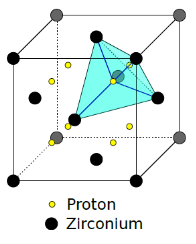
\includegraphics[width=0.4\textwidth]{ZrH.png} % Placeholder for image
    \caption{Crystal structure of Zirconium Hydride.}
    \label{fig:UZrH}
\end{figure}

The TRIGA fuel elements are cylindrical rods with a height of $70 cm$ and a diameter of $3.8 cm$, cladded with either aluminum (type 101) or stainless steel (type 103). The UZrH fuel contains $8\%$ uranium by weight, enriched to $19.95\%$. Graphite is used as both the upper and lower reflector, and burnable poisons or a central zirconium rod may be incorporated.

\begin{table}[H]
    \centering
    \renewcommand{\arraystretch}{1.5} % Increase row height
    \setlength{\tabcolsep}{10pt} % Adjust column spacing
    \begin{tabular}{|c|c|c|}
        \hline
        \textbf{} & \textbf{101-type} & \textbf{103-type} \\
        \hline
        \textbf{Cladding} & {Aluminium} & {304 SS} \\
        \hline
        \textbf{Zr:H Ratio} & {1:1} & {1:1.6} \\
        \hline
        \textbf{Other Features} & {2 disks of SmO$_3$} & {Zr Central Rod} \\
        \hline
    \end{tabular}
    \caption{Comparison of 101-type and 103-type fuel elements present in Pavia.}
    \label{tab:fuel_types}
\end{table}

For type 103 fuel elements, the Zr-H ratio is tuned to 1:1.6 to prevent any phase transitions in the crystal structure during transients. These fuel elements, located in the core's inner region, experience the most significant temperature variations.

\begin{figure}[H]
    \centering
    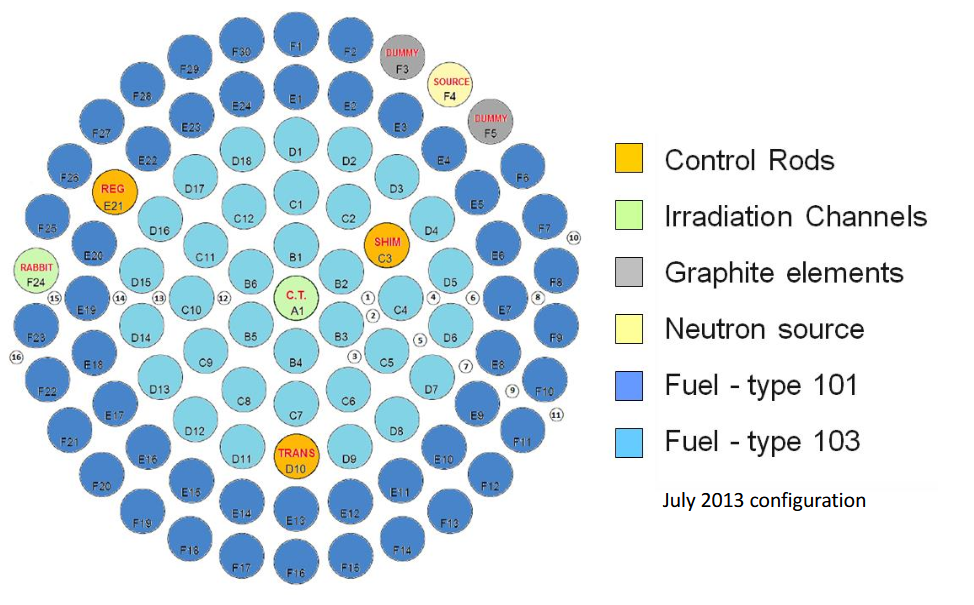
\includegraphics[width=0.7\textwidth]{core_structure.png} % Placeholder for image
    \caption{Current core structure of Triga reactor in Pavia.}
    \label{fig:core_structure}
\end{figure}

\paragraph{Control Rods} The TRIGA reactor's reactivity control system consists of three control rods:

\begin{itemize}
    \item \textbf{TRANSient rod} serves as the safety rod and remains outside the core during normal operation.
    \item \textbf{SHIM rod} compensates for large reactivity variations.
    \item \textbf{REGulating rod} is used for fine adjustments, managing small transients and stabilizing reactor power.
\end{itemize}

The position of the control rods is measured relative to full insertion, which corresponds to complete coverage of the active fuel length. Their position is displayed digitally on the control console in units known as \textit{digits}.

\begin{table}[H]
    \centering
    \renewcommand{\arraystretch}{1.5} % Increase row height
    \setlength{\tabcolsep}{10pt} % Adjust column spacing
    \begin{tabular}{|c|c|c|c|c|}
        \hline
        \textbf{Rod} & \textbf{Material} & \textbf{Composition} & \textbf{CRW} \\
        \hline
        SHIM & B$_4$C & $15.8\% ^{10} B$ & 3 $\sim$ 3.5 \$ \\
        \hline
        REG & B$_4$C & $15.8\% ^{10} B$ & 1 $\sim$ 1.5 \$ \\
        \hline
        TRANSIENT & Borated Graphite & $72\%C$ + $5.35\% ^{10} B$ + $21.7\% ^{11} B$ & 2 $\sim$ 2.5 \$ \\
        \hline
    \end{tabular}
    \caption{Control Rods and their characteristics}
    \label{tab:control_rods}
\end{table}


\section{Theoretical Background}

The theoretical and experimental framework of this study is based on the subcritical multiplication theory. This theory states that, in a nuclear reactor, a steady neutron flux can be maintained even in a subcritical state ($ k_{\text{eff}} < 1 $). 

This behavior is possible due to the presence of an external neutron source, which introduces an additional term in the neutron population equation of the Point Kinetics model:

\begin{equation}
\frac{dn}{dt} = \frac{\rho - \beta}{\Lambda} n + \sum_{i=1}^{6} \lambda_i C_i + \mathbf{q}
\end{equation}

\subsection{Neutron Sources}

Neutron sources play a crucial role in reactor operation, particularly in start-up procedures and in sustaining and monitoring the neutron flux under subcritical conditions. The design of neutron sources considers two primary parameters:
\begin{itemize}
    \item \textbf{Location} – Proper positioning ensures optimal neutron flux distribution.
    \item \textbf{Intensity} – Sufficient source strength is required to maintain detectable neutron levels.
\end{itemize}

Neutron sources can be either internal or external to the reactor core. 

In the first case, neutrons are generated by materials that are an integral part of the reactor, such as fissile material or through ($\alpha, n$) and ($\gamma, n$) reactions involving activated materials. 

On the other hand, an external source can rely on primary sources, such as spontaneous fission from elements like Californium ($^{252}\text{Cf}$), or on a combination of elements such as Radium and Beryllium, which produce neutrons via the $(\alpha, n)$ reaction. Additionally, secondary sources, such as Antimony-Beryllium, undergo the $(\gamma, n)$ reaction after irradiation, providing an alternative means of neutron generation.

For this study, the neutron source is external and primary, involving the ($\alpha, n$) reaction between Radium $^{226}\text{Ra}$ and Beryllium $^9\text{Be}$:

Radium undergoes \(\alpha\) decay with a half-life of \(\text{T}_{\frac{1}{2}} = 1600\) years:

\begin{equation}
^{226}_{88}\text{Ra} \rightarrow ^{222}_{86}\text{Rn} + \alpha    
\end{equation}

The emitted \(\alpha\) particles, with an energy of \(4.784\) MeV (branching ratio: \(94.5\%\)), interact with beryllium to produce neutrons via the following reaction:

\begin{equation}
\alpha + ^9_4\text{Be} \rightarrow ^{12}_6\text{C} + n
\end{equation}

Generated neutrons can reach a maximum energy of \(13\) MeV.


Even in a subcritical state, the neutrons injected into the system interact with the fuel, leading to a neutron population stabilization at an higher level than the source would provide by itself.

\subsection{Subcritical Multiplication Theory}

The subcritical multiplication theory can be analyzed within two different domains:

\subsubsection{Neutron Generations Domain}

When considering neutron generations, the neutron population follows a geometric progression with a ratio $ k $:

\begin{equation}
n = S (1 + k + k^2 + ... + k^n) \text{, where } S \text{ is the source magnitude}
\end{equation}

For a subcritical system $( k < 1 )$, the series converges to a finite asymptotic value:

\begin{equation}
n_{\infty} = \frac{S}{1 - k}
\end{equation}

This allows for the definition of the subcritical multiplication factor $ M $:

\begin{equation}
M = \frac{1}{1 - k}
\end{equation}

A useful parameter to quantify the deviation from criticality is the \textbf{subcritical margin}:

\begin{equation}
\text{Subcritical Margin} = 1 - k
\end{equation}

This margin influences both the subcritical multiplication factor $M$ and the number of generations required to reach the steady-state neutron population. Figure~\ref{fig:n_vs_gen} illustrates how neutron population varies over generations for different values of \( k \).

\begin{figure}[H]
    \centering
    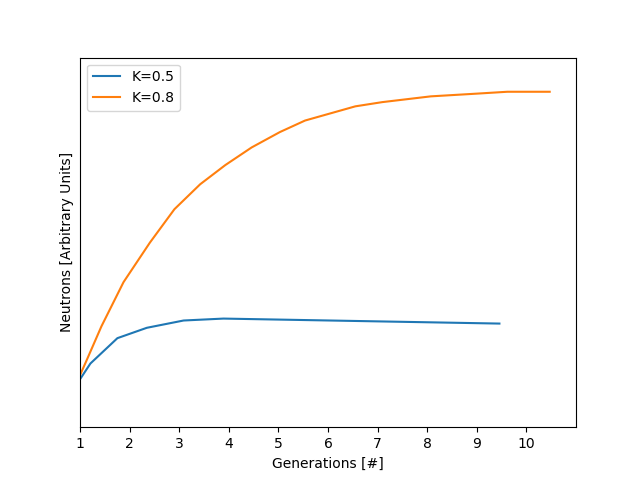
\includegraphics[width=0.7\textwidth]{neutron_population_generations.png} % Placeholder for plot
    \caption{Neutron population over generations for different values of $ k $.}
    \label{fig:n_vs_gen}
\end{figure}

\subsubsection{Time Domain}

When considering time as the primary domain, the Point Kinetics equations must be solved, incorporating the external neutron source term:

\begin{equation}
    \begin{cases}
        \frac{dn}{dt} = \frac{\rho - \beta}{\Lambda} n + \sum\limits_{i=1}^{6} \lambda_i C_i + q 
        = k \left( \frac{k-1}{k} + \rho - \beta \right) \frac{n}{l} + \sum\limits_{i=1}^{6} \lambda_i C_i + q \\[10pt]
        
        \frac{dC_i}{dt} = \frac{\beta_i}{\Lambda} n - \lambda_i C_i 
        = k \frac{\beta_i}{l} n - \lambda_i C_i
    \end{cases}
\end{equation}
    
The steady-state neutron population can be derived as:

\begin{equation}
    n_{\infty} = q \frac{l}{1 - k}
\end{equation}
Knowing the definiton of mean generation time and reactivity:
\begin{equation}
    \Lambda =\frac{l}{k}
\end{equation}
\hspace{1cm}
\begin{equation}
    \rho = \frac{k-1}{k}
\end{equation}
The steady-state neutron population can be expressed as:
\begin{equation}
    n_{\infty} = - q\frac{\Lambda}{\rho}
\end{equation}

Using the Laplace Transform, the time-dependent solution for $ n(t)$ is obtained:

\begin{equation}
n(t) = q \left(\mathbf{A_0} + A_1 e^{s_1 t} + A_2 e^{s_2 t}\right)
\end{equation}
The complete formulation is:
\begin{equation}
    n(t) = q \left( 
        -\frac{\Lambda}{\rho_0} 
        + \frac{\frac{\beta}{\rho_0}}{\frac{\lambda \rho_0}{\beta - \rho_0} + \frac{\beta - \rho_0}{\Lambda}} e^{\frac{\lambda \rho_0}{\beta - \rho_0} t} 
        + \frac{\frac{\lambda \Lambda}{\beta - \rho_0} - 1}{\frac{\lambda \rho_0}{\beta - \rho_0} + \frac{\beta - \rho_0}{\Lambda}} e^{-\frac{\beta - \rho_0}{\Lambda} t}
    \right)
\end{equation}

where $ s_1 $ and $ s_2 $ are the roots of the characteristic equation. The external source does not alter these exponential terms but introduces an integrator, leading to a \textbf{constant offset}.

The influence of the subcritical margin is evident in both the steady-state population and the settling time. Figure~\ref{fig:n_vs_time} presents the normalized neutron population over time following a sudden doubling of the neutron source strength for different values of $ k $.

\begin{figure}[H]
    \centering
    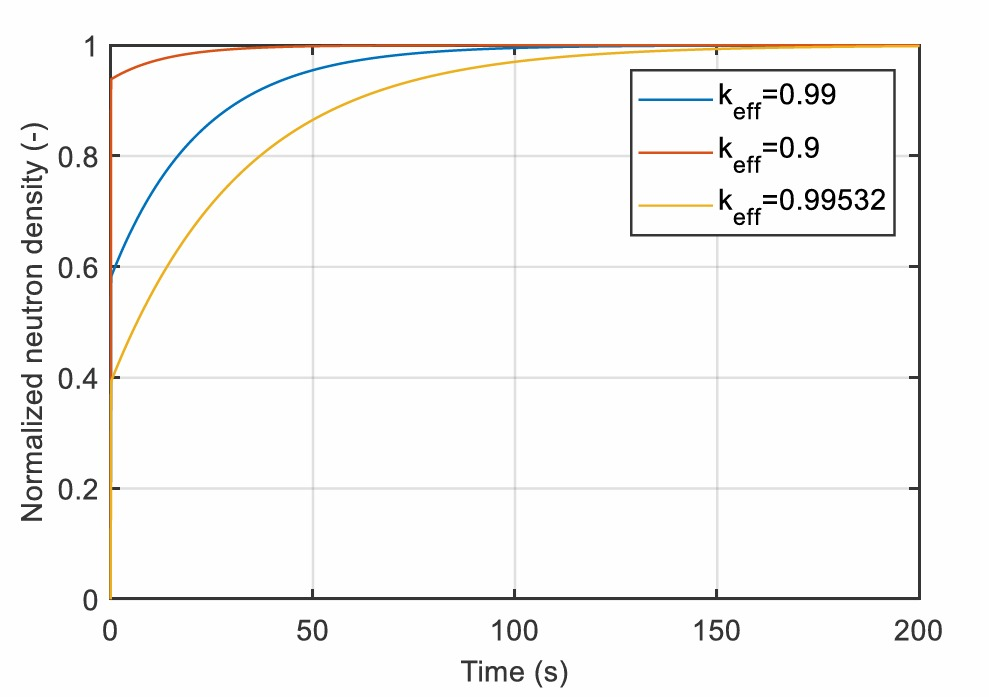
\includegraphics[width=0.7\textwidth]{neutron_population_time.jpg} % Placeholder for plot
    \caption{Time evolution of neutron population following a source strength doubling for different values of \( k \).}
    \label{fig:n_vs_time}
\end{figure}

This highlights two key effects of the multiplication factor:
\begin{itemize}
    \item As $ k $ approaches 1, the \textbf{settling time increases}.
    \item As  $ k $ increases, the \textbf{prompt jump} in neutron population decreases.
\end{itemize}

\subsubsection{Multiple Precursor Groups: In-Hour Equation}

This analysis assumes a single group of delayed neutron precursors for mathematical simplicity. However, a more accurate model should consider multiple precursor groups. The proper approach in such cases involves solving the \textit{In-Hour Equation}:

\begin{equation}
    \rho = \frac{\Lambda}{T} + \sum_{i=1}^{6} \frac{\beta_i}{1 + \lambda_i T}
\end{equation}

While the steady-state neutron population remains unchanged, incorporating multiple precursor groups results in a longer settling time compared to the single-group approximation.
\section{Monte Carlo Simulation}

A Monte Carlo simulation of the TRIGA Mark II reactor was developed using the SERPENT code. The core was modeled with reasonable fidelity to the real geometry, as illustrated in the following plots:

\begin{figure}[H]
    \centering
    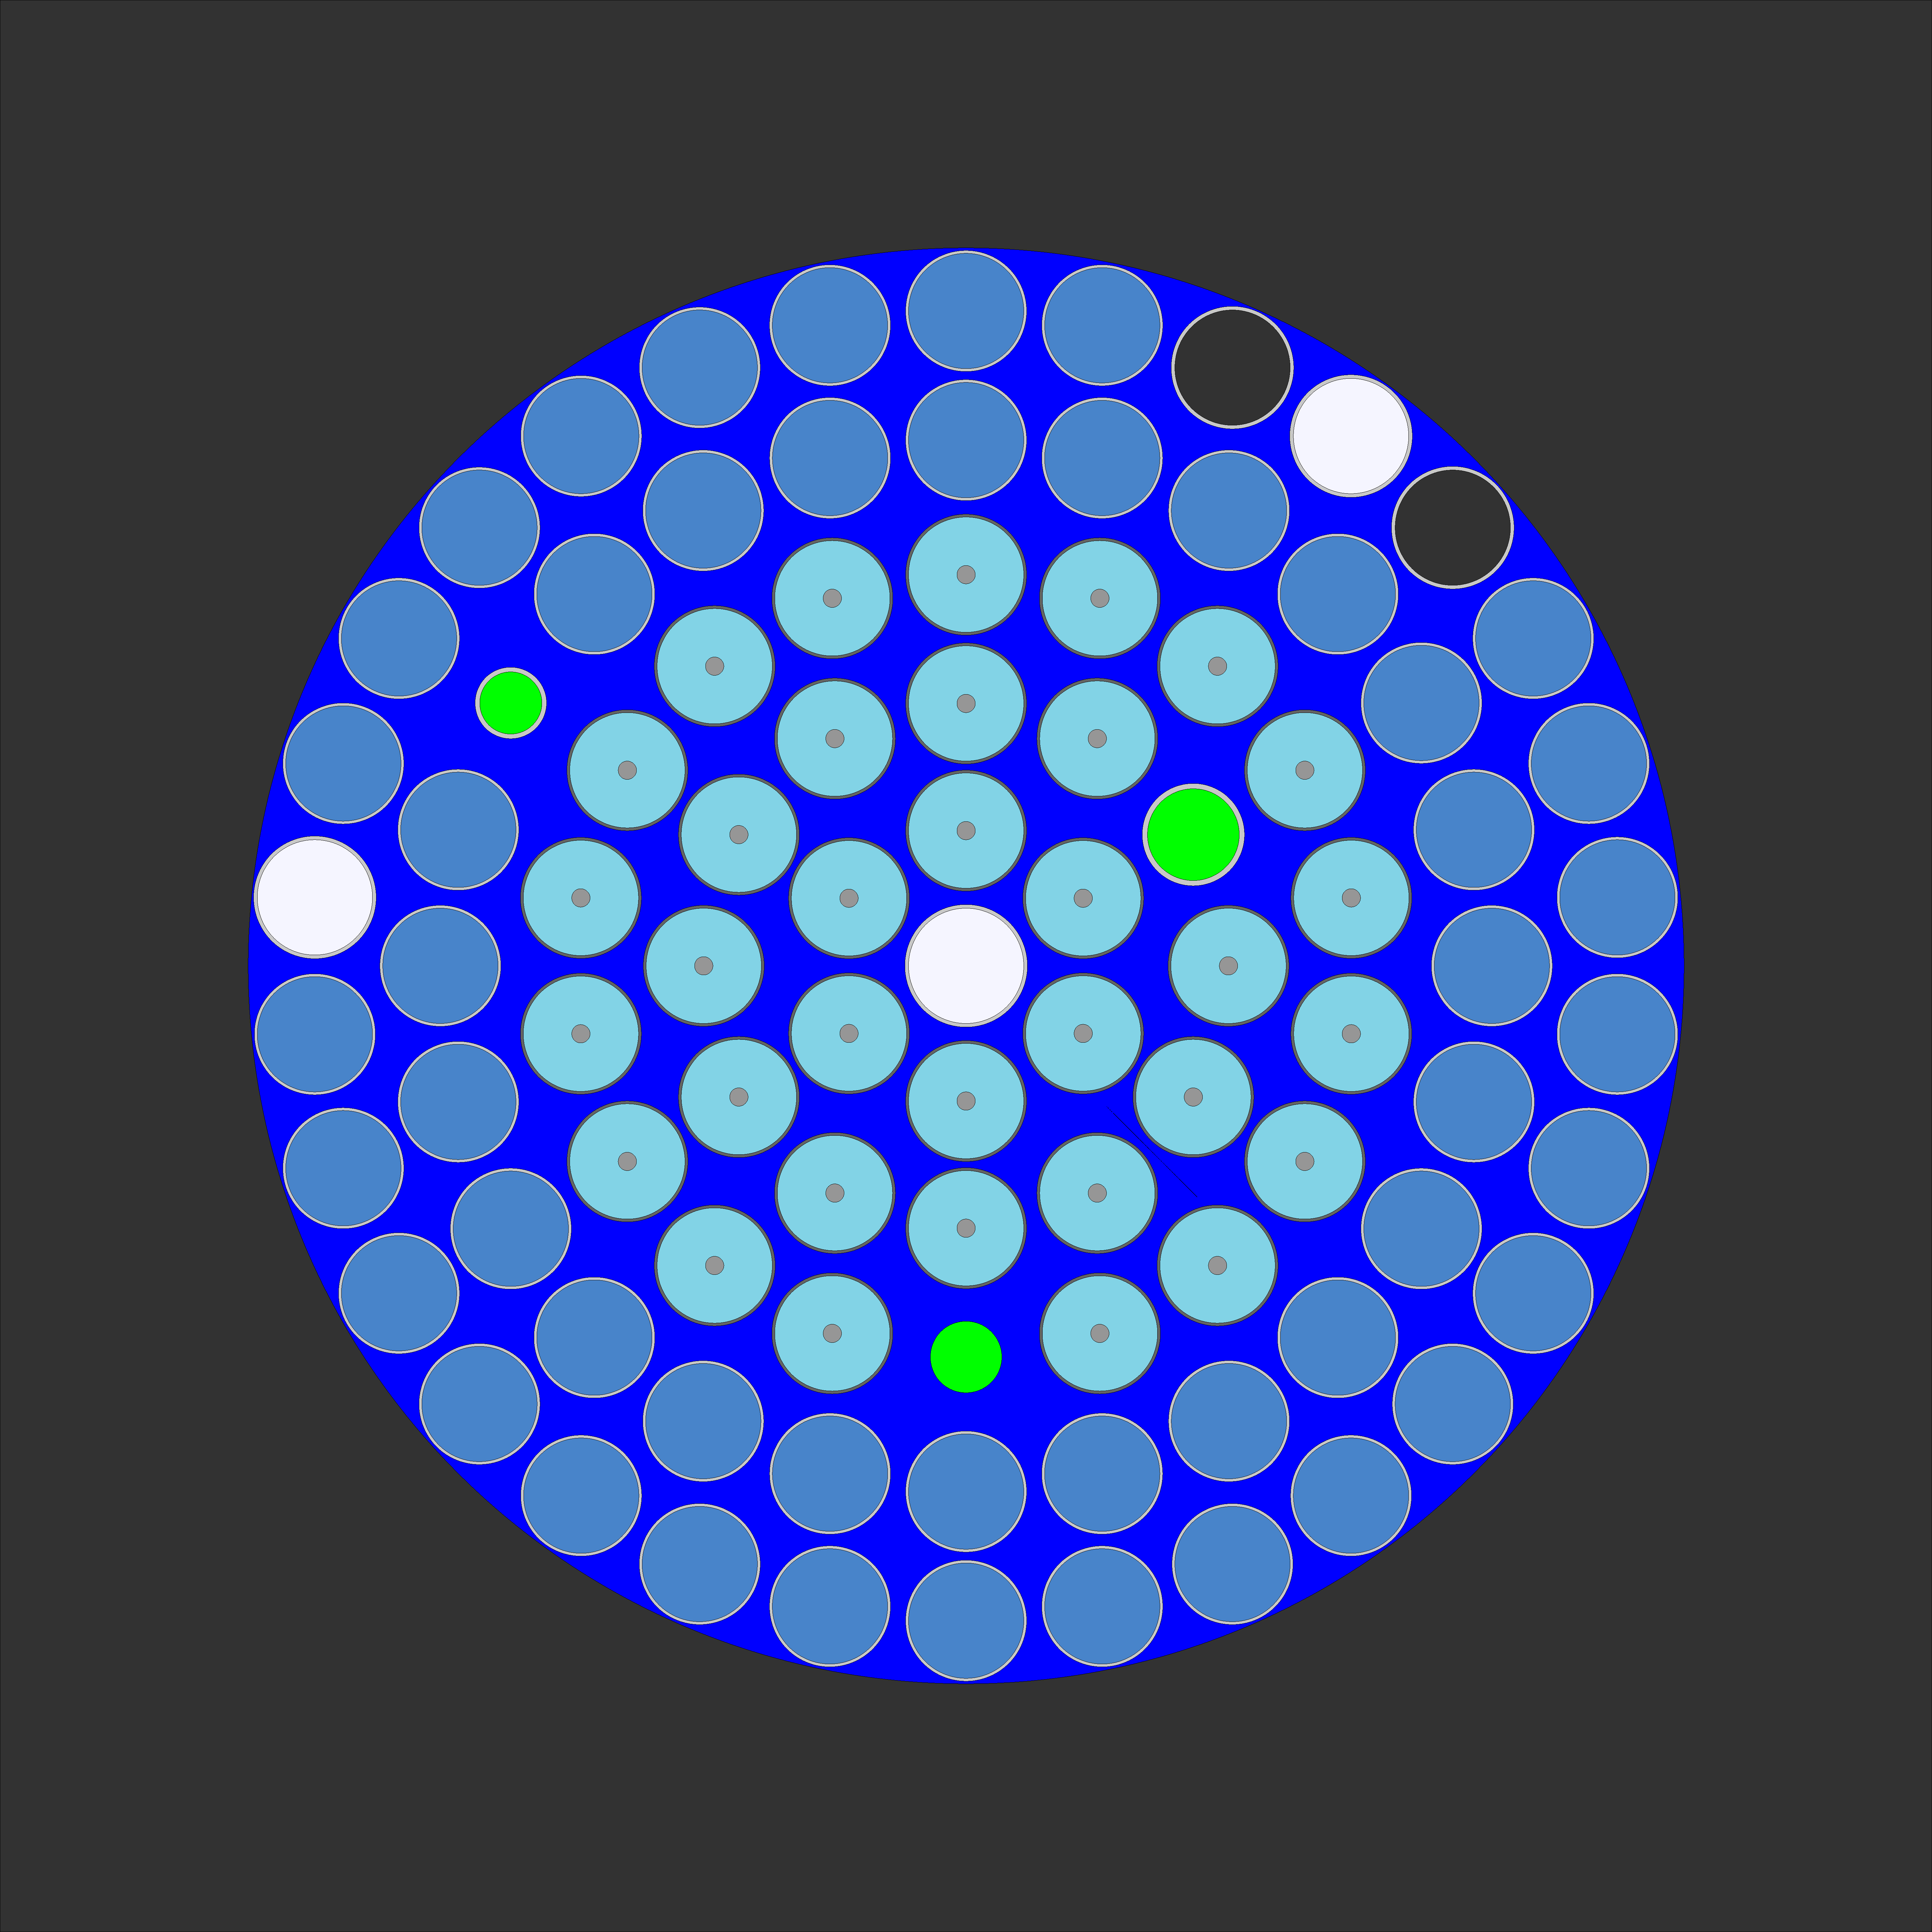
\includegraphics[width=0.45\textwidth]{TRIGA_Serpent_XY.png}
    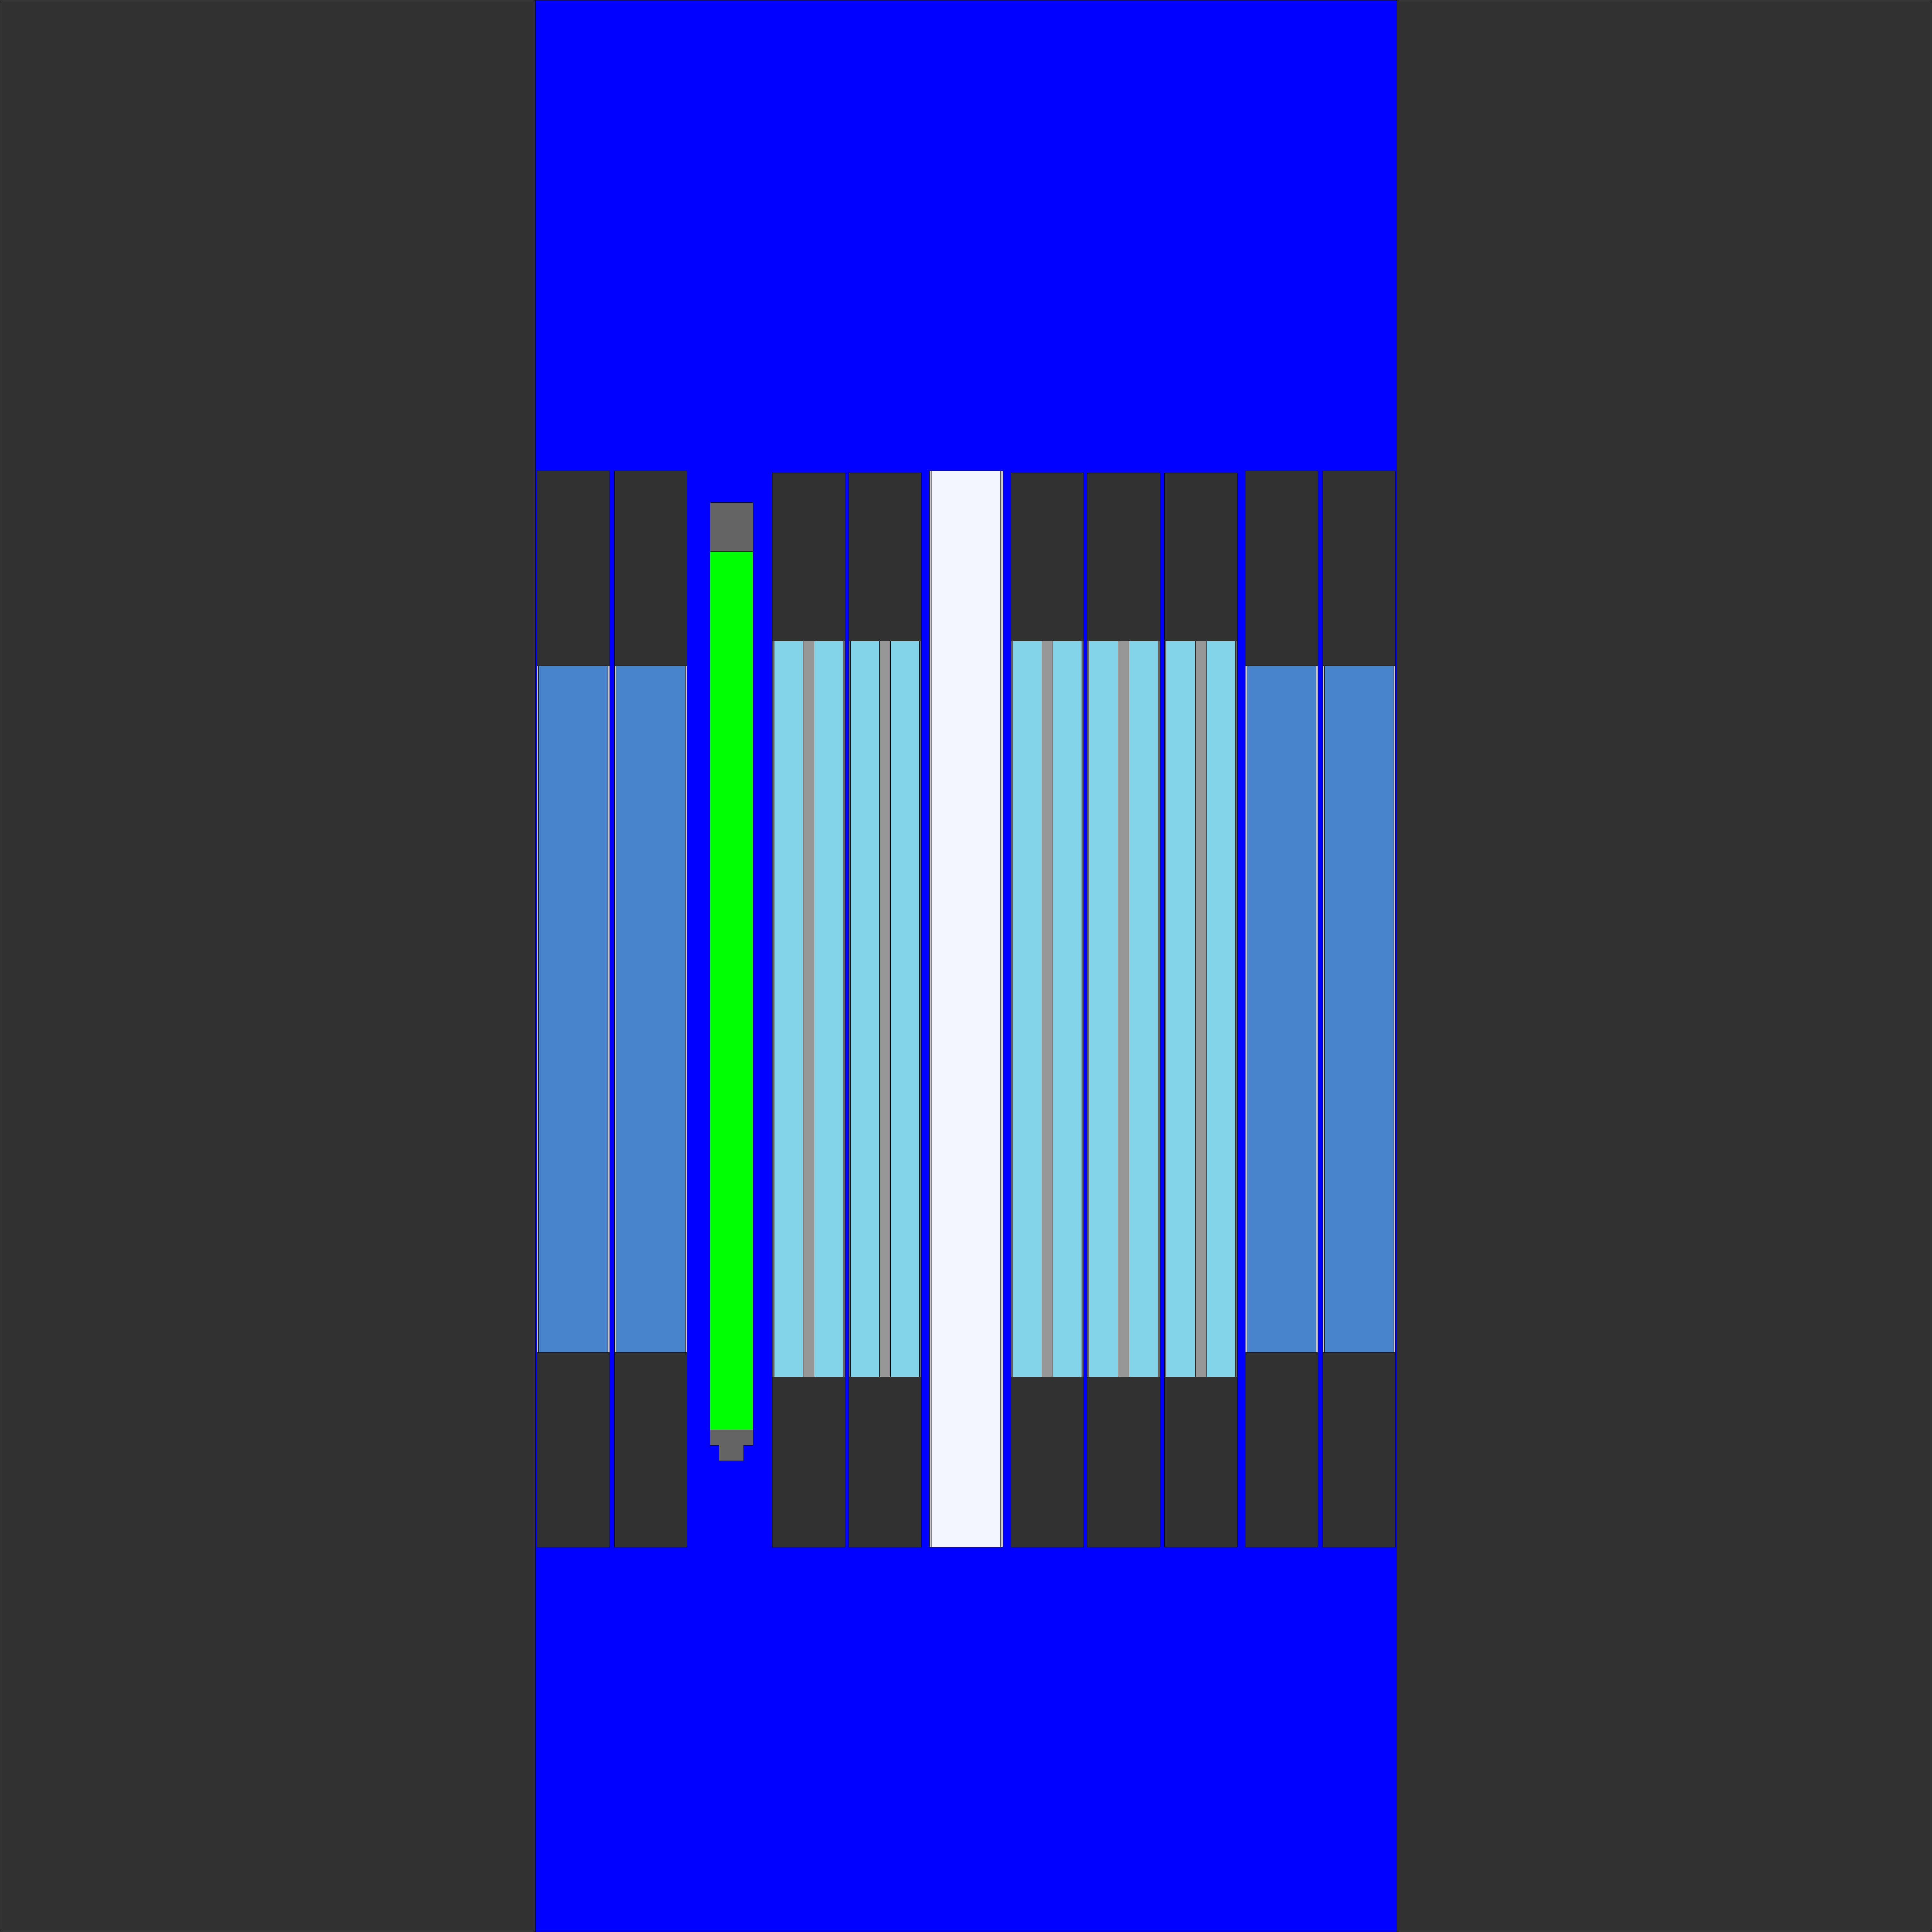
\includegraphics[width=0.45\textwidth]{TRIGA_Serpent_XZ.png}
    \caption{Horizontal and vertical section of the SERPENT geometry}
    \label{fig:triga_geometry}
\end{figure}

\subsection{Simulation Methodology}

The Monte Carlo model of the TRIGA core was first benchmarked against criticality calculations to ensure its validity, based on experience gained from the reactor period calibration of the REG control rod~\cite{Lorenzi2024}.

The simulation was initialized using the following command: \texttt{set pop 1000000 5000 20} which sets a population of 1 million neutrons, 5000 cycles, and 20 inactive cycles. 

The results were then normalized with: \texttt{set power 10} where power is in watts.

The obtained results indicate an overestimation of the control rod worth, where $k_{\text{eff, implicit}} $ from the simulation was taken as the result. The discrepancy in reactivity $\left( \rho = \frac{k-1}{k} \right)$ is shown in Table~\ref{tab:montecarlo_results}.

\begin{table}[h]
    \centering
    \begin{tabular}{|c|c|}
        \hline
        \textbf{Method} & \textbf{Result} \\
        \hline
        Montecarlo & $1.30 \pm 0.03\$$ \\
        Experimental & $1.26\$$ \\
        \hline
    \end{tabular}
    \caption{Control rod worth comparisons between Monte Carlo Criticality simulation and known experimental values, all values are in dollars $\left[ \$ \right]$.}
    \label{tab:montecarlo_results}
\end{table}

From these values, the overestimation can be quantified as:

\begin{equation}
\frac{\text{CRW}_{MC} - \text{CRW}_{\text{exp}}}{\text{CRW}_{\text{exp}}} = 3.34 \pm 2.55 \%
\end{equation}

which can be attributed to discrepancies between the model and the actual reactor core.

\subsection{Subcritical External Source Simulation}

After validating the core model, an external neutron source was introduced to simulate the subcritical calibration scenario. The neutron source (4.4 cm in height~\cite{Ponciroli2010}) was placed in the same channel as in the experimental setup, positioned at the bottom~\cite{Ponciroli2010}. To enable external source mode, the following parameters were set:
\begin{lstlisting}
src 1 n sm Vacuum_Source
sb 11
...
\end{lstlisting}

Which defines a neutron source in the specified material (vacuum for simplicity).
The energy was defined as a histogram distribution in 11 bins, which was based on literature data~\cite{Geiger1964}.
Delayed neutrons were explicitly considered (as they are neglected by default): \texttt{set delnu 1}.

The normalization condition was set based on the source emission rate: \texttt{set srcrate 1e7}.

The following parameters were set to define the number of neutrons and batches in the external source simulation: \texttt{set nps 100000 50}.

To prevent excessive memory usage, constraints were defined for the maximum and minimum time a neutron can be scored~\cite{SerpentMC2013}:

\begin{lstlisting}
    set tcut 3e-3
    set cfe -1 6E-6
\end{lstlisting}

All other parameters and geometry remained unchanged.

\subsection{Simulated Conditions}

The following control rod configurations were simulated:

\begin{table}[H]
    \centering
    \begin{tabular}{|c|c|}
        \hline
        \textbf{Configuration} & \textbf{\( k_{\text{eff}} \)} \\
        \hline
        All in & $0.962708 \pm 0.00127$ \\
        Regulating rod out & $0.986959 \pm 0.00036$ \\
        Shim rod out & $0.974998 \pm 0.00069$ \\
        Transient rod out & $0.980734 \pm 0.00069$ \\
        \hline
    \end{tabular}
    \caption{Simulated core configurations and resulting $ k_{\text{eff}} $ values.}
    \label{tab:keff_values}
\end{table}

From these values, the control rod worth can be calculated as:

\begin{equation}
\rho _i = \frac{k_{\text{eff}, i} - 1}{k_{\text{eff}, i}}
\end{equation}

\begin{equation}
\text{CRW}_i = \rho_{i} - \rho_{\text{all in}} 
\end{equation}

\subsection{Comparison with Experimental Data}

The results from the Monte Carlo simulations exhibit a systematic overestimation of control rod worth compared to experimental measurements. This discrepancy can be attributed to various factors, including:

\begin{itemize}
    \item Differences between the modelled and actual core configurations.
    \item Inaccuracy in neutron source energy spectra.
    \item Uncertainties in nuclear data libraries.
    \item Computational limits imposed on the simulation.
\end{itemize}

\begin{table}[h]
    \centering
    \begin{tabular}{|c||c|c|c||c|c|c||c|c|c|}
        \hline
        \multicolumn{1}{|c||}{} & \multicolumn{3}{c||}{\textbf{REG}} & \multicolumn{3}{c||}{\textbf{TRANS}} & \multicolumn{3}{c|}{\textbf{SHIM}} \\
        \hline
        \multicolumn{1}{|c||}{} & Min & Result & Max & Min & Result & Max & Min & Result & Max \\
        \hline
        \textbf{MC} & $1.58$ & $1.79 \pm 0.21$ & $2.00$ 
        & $2.41$ & $2.62 \pm 0.21$ & $2.83$ 
        & $3.31$ & $3.50 \pm 0.19$ & $3.69$ \\
        \hline
        \textbf{Ref} & \multicolumn{3}{c||}{$1.26$} & \multicolumn{3}{c||}{$2.23$} & \multicolumn{3}{c|}{$3.22$} \\
        \hline
    \end{tabular}
    \caption{Control rod worth comparisons between Monte Carlo (MC) simulations and reference experimental values (Ref) provided by LENA, all values are in dollars $\left[ \$ \right]$.}
    \label{tab:cr_worth}
\end{table}

\subsection{Observations}

The Monte Carlo model provides a valuable tool for evaluating control rod calibration procedures. Although the raw simulation results show a slight overestimation, the overall consistency between Monte Carlo results and experimental data supports the validity of the subcritical control rod calibration method used in this study.

Further refinement of the Monte Carlo model could improve accuracy. Particular attention should be given to:

\begin{itemize}
    \item Refining the simulation time constraints.
    \item Improving the representation of the reactor’s real-state conditions.
    \item Enhancing the accuracy of neutron source modelling.
\end{itemize}
\section{Experimental Campaign}

The experimental campaign aims to validate the proposed model, which establishes a relationship between reactivity insertion due to control rod movement and a measurable parameter. In this case, the chosen parameter is the counting rate of a fission chamber.

The use of a fission chamber is necessary due to the low reliability of power measurements at extremely low levels and the difficulty in precisely determining the neutron source intensity. By employing this method, variations in neutron flux between different control rod configurations can be inferred.

Since the efficiency of the source-counting system and the exact neutron flux are unknown, this approach is considered an \textit{approximate method}. These uncertainties are managed by computing a calibration factor associated with the fission chamber.
\subsection{From Differential to Integral Reactivity Worth}

The differential reactivity curve of a control rod can be, in principle, determined by exploiting the relationship between the multiplication factor $k$ and the subcritical multiplication factor $M$, which links the neutron source intensity to the steady-state neutron population in the core.

By evaluating the reactivity difference between successive extraction steps, the differential reactivity worth can be estimated as:

\begin{equation}
\Delta \rho = \rho_{i+1} - \rho_i
\end{equation}

However, due to the high uncertainty associated with small step extractions, this experiment was limited to a single extraction step. For each control rod, the reactivity difference was determined by comparing the fully inserted and fully extracted configurations, providing a more robust estimation of its integral worth.

\subsection{Calibration Factor Calculation}

At steady state, the counting rate is given by:

\begin{equation}
\dot{C}_{\infty} = \alpha \phi_s M
\end{equation}

where $ \alpha \phi_s $ is the calibration factor, which must be determined by comparison with a known reference condition. The relationship between two different counting rate measurements is expressed as:

\begin{equation}
\gamma = \frac{\dot{C}_{\infty,known}}{\dot{C}_{\infty,ref}} = \frac{M_{known}}{M_{ref}} = \frac{1-k_{ref}}{1-k_{known}}
\end{equation}

The calibration factor is computed by comparing the reference condition (all rods inserted, corresponding to a control rod worth of zero) with a known condition obtained from previous calibration experiments. The steps involved are:


\begin{align}
    \gamma &= \frac{\dot{C}_{\text{known}}}{\dot{C}_{\text{ref}}} \notag \\
    & \downarrow  \notag \\
    \rho_{\text{ref}} &= - \frac{CRW_{\text{ref}} - 1}{2} - \frac{1}{2} \sqrt{\left( CRW_{\text{ref}} - 1\right)^2 + 4 CRW_{\text{ref}} \frac{\gamma}{\gamma - 1}} \notag \\
    & \downarrow  \notag \\
    k_{\text{ref}} &= \frac{1}{1 - \rho_{\text{ref}}} \notag \\
    & \downarrow  \notag \\
    M_{\text{ref}} &= \frac{1}{1 - k_{\text{ref}}} \notag \\
    & \downarrow  \notag \\
    \alpha \phi_s &= \frac{\dot{C}_{\text{ref}}}{M_{\text{ref}}}
\end{align}

This highlights the necessity of prior calibration for at least one control rod to obtain meaningful results.

\subsection{Control Rod Worth Estimation}

Once the steady-state counting rate is measured and the calibration factor is determined, the subcritical multiplication factor $ M $, the effective multiplication factor $ k $, and reactivity $ \rho $ can be computed as follows:
\begin{align}
    M_i &= \frac{\dot{C}_i}{\alpha \phi_s} \notag \\
    & \downarrow \notag \\
    k_i &= 1 - \frac{1}{M_i} \notag \\
    & \downarrow \notag \\
    \rho_i &= \frac{k_i - 1}{k_i} \notag \\
    & \downarrow \notag \\
    \text{CRW} &=  \rho_i -\rho_{\text{ref}} \quad [\text{pcm}]
\end{align}

This methodology ensures a systematic approach for determining the reactivity worth of each control rod based on measured neutron counting rates.


\begin{tcolorbox}[boxstyle2]
    \textbf{Application to SHIM Rod Calibration}:
    The experimental procedure provides a rapid but approximate determination of the integral control rod worth. Given the subcritical nature of all procedural steps, this method can also be applied to calibrate the SHIM control rod. This is particularly relevant since alternative calibration techniques, such as the reactor period method, may encounter difficulties due to the high reactivity worth of the SHIM rod.
\end{tcolorbox}


\subsection{Instrumentation}

The experimental setup includes the following components:

\begin{itemize}
    \item TRIGA Reactor.
    \item Control rods and control panel.
    \item Neutron source: Radium-Beryllium, activity $2~Ci$, neutron emission rate: $10^7 \frac{n}{s}$, placed in the outermost ring (F).
    \item Fission chamber and its counting chain, operated in pulse mode. A timer is incorporated for setting the measurement time.
    \item Previous calibration data of the control rods.
\end{itemize}

The reactor is managed by a qualified operator.

\subsection{Procedure}

\begin{enumerate}
    \item \textbf{Bring the reactor to a cold subcritical condition with all control rods inserted.}  
    Ensure that the fuel temperature is close to room temperature to confirm a ``cold'' condition.  
    Verify that the reactor is in a ``clean'' state by checking radioactivity and conductivity measurements of the cooling water.

    \item \textbf{Measure the natural background counting rate.}  
    This measurement is performed before inserting any neutron source.

    \item \textbf{Insert the Ra-Be source into the F ring and measure the counting rate.}  
    This configuration serves as the reference measurement.

    \item \textbf{Calculate the calibration factor by comparison with a known configuration.}  
    The previous calibration of any control rod can be used. For example, if the REG calibration is employed, the measurement should be taken with the REG rod fully extracted while keeping all other control rods inserted.

    \item \textbf{Perform a control rod extraction step.}  
    Any control rod can be calibrated using this approach. For this specific experiment, only a single extraction step is performed, where the control rod is fully removed.

    \item \textbf{Wait for the steady-state condition and measure the counting rate.}  
    Steady-state achievement is confirmed by monitoring power behavior.  
    A fixed measurement time of 100 seconds is used, with multiple measurements taken to improve statistical accuracy.

    \item \textbf{Compute the relevant parameters from the recorded data.} $M$, $k$, and finally $\rho$.

    \item \textbf{Repeat Step 6 for successive extraction steps.}  
    Not required in this specific experiment, as only a single extraction step is considered.
\end{enumerate}


\subsection{Results Collection}

Following the described procedure, experimental data were recorded for all possible control rod configurations.

\begin{table}[H]
    \centering
    \begin{tabular}{|c|c|c|c|c|}
        \hline
        \multirow{18}{*}{\rotatebox{90}{\textbf{Integral Counts}}} 
        & All in & Reg out & Trans out & Shim out \\
        \cline{2-5}
        & $60$  & $76$  & $167$  & $261$  \\
        & $71$  & $69$  & $123$  & $303$  \\
        & $92$  & $102$ & $156$  & $211$  \\
        & $59$  & $90$  & $122$  & $219$  \\
        & $59$  & $87$  & $214$  & $228$  \\
        & $77$  & $111$ & $119$  & $243$  \\
        & $52$  & $67$  & $160$  & $332$  \\
        & $65$  & $89$  & $164$  & $239$  \\
        & $45$  & $96$  & $159$  & $244$  \\
        & $68$  & $93$  & $108$  & $241$  \\
        & $37$  & $80$  &       &  \\
        & $52$  & $80$  &       &  \\
        & $72$  & $85$  &       &  \\
        & $64$  & $85$  &       &  \\
        & $67$  & $91$  &       &  \\
        & $68$  & $86$  &       &  \\
        & $66$  & $101$ &       &  \\
        & $66$  & $113$ &       &  \\
        & $64$  & $80$  &       &  \\
        & $54$  & $90$  &       &  \\
        \hline
        $\langle C \rangle \pm \sigma_{\langle C \rangle}$ & $62.9 \pm 1.8$  & $88.6 \pm 2.1$  & $149.2 \pm 3.9$  & $252.1 \pm 5.0$  \\
        $\dot{C} \pm \sigma_{\dot{C}}$ & $0.63 \pm 0.02$  & $0.89 \pm 0.02$  & $1.49 \pm 0.04$  & $2.52 \pm 0.05$  \\
        \hline
    \end{tabular}
    \caption{Counts, average counts, standard deviation, and counting rate for different control rod configurations. Data for TRANS and SHIM rod were taken by half of the groups during the data collection}
    \label{tab:results}
\end{table}


The raw data consists of $N$ integral neutron counts $C$, each measurement performed over a 100-second interval $\left(\Delta t\right)$. The count rate $\dot{C}$ and its error were computed using the following formulas:

\begin{equation}
    \langle C \rangle = \frac{\sum{C}}{N}
\end{equation}

\begin{equation}
    \sigma_{\langle C \rangle} = \sqrt{\frac{\langle C \rangle}{N}}
\end{equation}

\begin{equation}
\dot{C} = \frac{\langle C \rangle}{\Delta t}
\end{equation}

\begin{equation}
\sigma_{\dot{C}} = \frac{\sigma_{\langle C \rangle}}{\Delta t}
\end{equation}


\section{Data Analysis}

Based on the collected data and the outlined procedure, the control rod worth (CRW) is estimated for each control rod. The results are then converted into dollars by normalizing with the known value of the delayed neutron fraction $\beta$:

\begin{equation}
\text{CRW} \ [\$] = \frac{\text{CRW} \ [\text{pcm}]}{\beta}
\end{equation}

The values computed by using the REG as a reference are reported in the following table:

\begin{table}[H]
    \centering
    \begin{tabular}{|c|c|c|c|}
        \hline
        & \text{Reg} & \text{Trans} & \text{Shim} \\
        \hline
        $\alpha \phi_s$ & \multicolumn{3}{c|}{$0.018957 \pm 0.002415$} \\
        \hline
        $M$ & $46.71 \pm 6.06$ & $78.71 \pm 10.25$ & $132.99 \pm 17.18$ \\
        \hline
        $K$ & $0.9786 \pm 0.0028$ & $0.9873 \pm 0.0017$ & $0.9925 \pm 0.00097$ \\
        \hline
        $\rho$ & $-0.0219 \pm 0.0029$ & $-0.0129 \pm 0.0017$ & $ -0.00758 \pm 0.00099$ \\
        \hline
        $CRW$ & $1.26 \pm 0.70$ & $2.49 \pm 0.62$ & $3.22 \pm 0.59$ \\
        \hline
    \end{tabular}
    \caption{Table of calculated values for different control rods, using experimental calibration results.}
    \label{tab:crw_results}
\end{table}

\subsection{Calibration with different reference values}

The same procedure can be applied using the previously obtained calibration of the SHIM and TRANS rods, leading to the following results:

\begin{table}[H]
    \centering
    \begin{tabular}{|c|c|c|c|}
        \hline
        \textbf{Reference Calibration}& \textbf{Calibration Factor $\alpha \phi_s$} & \textbf{Control Rod}  & \textbf{CRW [\$]} \\
        \hline
        \multirow{3}{*}{REG Rod} 
            &                             & REG      & $1.26 ± 0.70$ \\
            & $0.018957 \pm 0.002415$     & TRANS    & $2.49 ± 0.62$ \\
            &                             & SHIM     & $3.22 ± 0.59$ \\
        \hline
        \multirow{3}{*}{TRANS Rod} 
            &                             & REG      & $1.13 ± 0.39$ \\
            & $0.018963 \pm 0.001155$     & TRANS    & $2.23 ± 0.35$ \\
            &                             & SHIM     & $2.88 ± 0.33$ \\
        \hline
        \multirow{3}{*}{SHIM Rod} 
            &                             & REG      & $1.26 ± 0.36$ \\
            & $0.017027 \pm 0.001325$     & TRANS    & $2.50 ± 0.31$ \\
            &                             & SHIM     & $3.22 ± 0.30$ \\
        \hline
    \end{tabular}
    \caption{Calibration factors and control rod worth (CRW) values for different reference calibrations.}
    \label{tab:calibration_results}
\end{table}

This analysis allows the estimation of control rod worth using different reference calibrations, ensuring consistency and reliability in the evaluation of reactivity control.


\subsection{Considerations}

The control rod selected as the reference for calibration inherently produces exact results for its own computed worth. However, when using one control rod as a reference to calibrate others, the accuracy of the results is influenced by statistical uncertainties.

It is important to note that the similarity between the values obtained using the REG rod as a reference and those obtained using the SHIM rod is purely coincidental. This is evident from the significantly larger associated uncertainties in the first case.

A consistent trend observed in the results is that the control rod with the lowest reactivity worth exhibits the highest relative error. This occurs because the difference in neutron population between the fully inserted and fully extracted configurations is smaller, leading to lower counting rates. Consequently, the measurement becomes more susceptible to statistical fluctuations.

For the same reason, the lowest uncertainties were found when the SHIM rod was used as a calibration reference, while the highest uncertainties were observed when the REG rod was used.

Finally, a notable observation is the generally high relative errors in the computed values. This outcome is expected, as the recorded counting rates are relatively low. Due to Poisson statistics, the relative uncertainty increases as the magnitude of the measurement decreases. Potential improvements to mitigate this issue include increasing the measurement duration, using a more sensitive detector, or optimizing detector placement.


\subsection{Effect of Reactor Clean state on Measurements}

If the reactor is not in a clean condition, it implies the accumulation of neutron poisons due to the buildup of fission products. This accumulation leads to a reduction in the number of available neutrons, accordingly decreasing detection efficiency.

Since the distribution of neutron poisons follows the neutron flux, certain regions of the core will exhibit higher concentrations of poisons. This variation affects the flux distribution, consequently altering control rod effectiveness. For instance, the SHIM rod, which has the highest control rod worth (CRW) due to its location in a high-flux region, will experience greater poison production. As a result, its effectiveness might be noticeably impacted.

A quantitative estimation of this effect could be obtained by analyzing the reduction in the SHIM rod's CRW (provided it is not used as a reference). Any observed decrease in its worth could be attributed to negative reactivity insertion due to poison buildup. However, for such an analysis to be reliable, it is essential to first validate the method under clean reactor conditions to establish a baseline reference.

\subsection{Sources of Error and Uncertainties}

Before discussing the details of error propagation, it is important to acknowledge that since the counting rate was obtained using a fission chamber, the calibration values determined in this experiment are only valid for the present conditions. For any future experiments, the calibration factor must be recomputed to account for potential degradation due to the burnup of fissile material in the fission chamber. However, during the short duration of the measurements, the burnup is assumed to be negligible.

\paragraph{Neglected Uncertainties} Several uncertainties were not explicitly accounted for in our analysis, including:

\begin{itemize}
    \item Uncertainty in $\beta$ from Monte Carlo simulations.
    \item Errors in the measurement chain beyond intrinsic Poisson uncertainty (e.g., timing errors).
    \item Uncertainty in the known CRW values.
    \item Shadowing effects, which were not considered.
\end{itemize}

\subsubsection{Statistical Treatment and Error Propagation}

The raw data analysis was performed using Poisson statistics, where the standard deviation of the counts is given by:

\begin{equation}
\sigma_{C} = \sqrt{C}
\end{equation}

To propagate errors through subsequent calculations, the root sum square (RSS) method was employed:

\begin{equation}
\sigma_f = \sqrt{\sum_{i} \left( \frac{\partial f}{\partial x_i} \sigma_{x_i} \right)^2}
\end{equation}

where $\sigma_f$ is the propagated uncertainty of a function $f$, and $\sigma_{x_i}$ represents the uncertainty of each variable $x_i$.

\subsubsection{Numerical Implementation}

This error propagation methodology was implemented in Python, where the partial derivatives were computed numerically based on ~\cite{Moffat1988}. 
The implementation in Python can be found in the appendix~\ref{appendix:python_code}

\section{Conclusions}
This study provided valuable insights into control rod calibration in the TRIGA Mark II reactor, 
demonstrating the effectiveness of the subcritical multiplication method while maintaining safe conditions. 

Monte Carlo simulations showed a systematic overestimation of control rod worth, likely due to modeling approximations, 
though experimental results remained consistent with theoretical expectations. 
The choice of reference rod significantly influenced uncertainties, with the Shim rod yielding more precise measurements. 

Future improvements should focus on refining Monte Carlo modeling approaches and enhancing experimental procedure to further reduce uncertainties.

\section*{Acknowledgments}
This report was prepared as part of the Experimental Nuclear Reactor Kinetics course by Professor Stefano Lorenzi at Politecnico di Milano (2024/25)~\parencite{Lorenzi2024}.

The authors thank the Serpent community for providing valuable resources~\parencite{SerpentWiki, SerpentForum}. 

All code and auxiliary data analysis are publicly available on GitHub~\parencite{PagliucaGithub}.

\appendix
\section{Python Implementation for Error Propagation} \label{appendix:python_code}

\begin{lstlisting}[language=Python]
    class Measurement:
    def __init__(self, value, uncertainty):
        if uncertainty < 0:
            raise ValueError("Uncertainty must be non-negative")
        self.value = value
        self.uncertainty = uncertainty
        # String representation
    def __str__(self):
        return f"{self.value:.6g} ± {self.uncertainty:.6g}"

    def rss(func, *measurements):
    # Extract nominal values for function evaluation
    nominal_values = [m.value for m in measurements]
    value = func(*nominal_values)
    
    # Numerical differentiation and uncertainty propagation
    epsilon = 1e-8  # Small step for finite differences
    squared_uncertainty = 0

    for i, m in enumerate(measurements):
        perturbed_values_plus = nominal_values[:]
        perturbed_values_minus = nominal_values[:]
        perturbed_values_plus[i] += epsilon
        perturbed_values_minus[i] -= epsilon

        # Partial derivative approximation
        df_dxi = (func(*perturbed_values_plus) - func(*perturbed_values_minus)) / (2 * epsilon)
        
        # Add contribution to total uncertainty
        squared_uncertainty += (df_dxi * m.uncertainty) ** 2

    total_uncertainty = math.sqrt(squared_uncertainty)
    
    # Return the resulting measurement
    return Measurement(value, total_uncertainty)

    # Example usage
    k_val = Measurement(1.24, 0.02)
    rho = rss(lambda k: (k-1)/k, k_val)
    print(rho) 
    # Output: 0.193548 ± 0.0130073

\end{lstlisting}

\newpage

% Bibliography
\printbibliography

\end{document}